
%(BEGIN_QUESTION)
% Copyright 2011, Tony R. Kuphaldt, released under the Creative Commons Attribution License (v 1.0)
% This means you may do almost anything with this work of mine, so long as you give me proper credit

Each of these illustrations shows an RTD connected improperly to a temperature transmitter.  Correct the mis-wiring, and also calculate the temperature ``seen'' by the transmitter given the improper sensor connections:

$$\includegraphics[width=15.5cm]{i03417x01.eps}$$

$T_{indicated}$ with incorrect 3-wire RTD wiring = \underbar{\hskip 50pt}

\vskip 20pt

$T_{indicated}$ with incorrect 4-wire RTD wiring = \underbar{\hskip 50pt}

\vskip 10pt

Identify whether or not these measurement errors could be compensated by recalibrating the transmitter.  If so, identify which calibration adjustment (zero or span) would have to be changed on the analog transmitter.

\vfil 

\underbar{file i03417}
\eject
%(END_QUESTION)





%(BEGIN_ANSWER)

This is a graded question -- no answers or hints given!

%(END_ANSWER)





%(BEGIN_NOTES)

255 deg F = 147.53 ohms (from RTD table)

\vskip 10pt

When identifying how to properly connect an RTD to a transmitter, remember that the rectangle symbol printed near the screw terminals on the body of the transmitter represents the resistive element of the RTD (i.e. which terminals that element should be connected to), while the connected lines represent those RTD leads that are electrically common (equipotential) to each other.  If you connect the RTD to the transmitter in exactly the manner shown by this symbology, the system should function properly.

\vskip 10pt

The problem with the 3-wire transmitter circuit is that the RTD is connected between terminals 2 and 3 while it should be connected between terminals 1 and 2 (where the rectangle element is shown printed on the transmitter face).  The common wires should be terminals 2 and 3, which is where you should place your jumper wire near the RTD.

The problem with the 4-wire transmitter circuit is that the jumpers are installed at the wrong end of the cable.  When placed at the transmitter's terminals, the transmitter has no way of compensating for lead resistance.  If the jumpers are placed between 1-2 and between 3-4 at the RTD, the transmitter is able to "use" the two outer conductors to sense voltage dropped by the RTD's resistive element right at the RTD and thereby compensate for lead resistance.

$$\includegraphics[width=15.5cm]{i03417x02.eps}$$

$T_{indicated}$ with incorrect 3-wire RTD wiring = \underbar{\bf Full downscale} (transmitter sees only 1.7 ohms of RTD resistance, and over 125 ohms of wire resistance!)

\vskip 10pt

$T_{indicated}$ with incorrect 4-wire RTD wiring = \underbar{{\bf 263 deg F} or {\bf 128.3 deg C}} (transmitter sees 149.23 ohms of RTD resistance)

\vskip 10pt

The 4-wire circuit's error is a {\it zero shift}, and therefor could be compensated by readjusting the ``zero'' screw (assuming wire resistance does not change substantially).  The 3-wire circuit's error is such that it doesn't even respond to process temperature at all, and no compensation is possible!

%INDEX% Calibration errors, identifying
%INDEX% Measurement, temperature: RTD connections

%(END_NOTES)


